\section{Experiments}
\label{sec:experiments}

We ask four questions: (Q1) does learned friction outperform always-executing? (Q2) does the hierarchical factoring (gate+selector) help or hurt relative to a flat 6-way softmax? (Q3) can RL exploit the safety reward in ways that a random or always-execute policy cannot? (Q4) what happens with real API calls rather than the rule-based simulator?

\subsection{Setup}

\paragraph{Tasks.}
We reuse the five ambiguity categories from \textsc{Ponder} \cite{ponder2026}: referential ($10$ tasks), trajectory ($10$), implicit-precondition ($8$), contextual-safety ($8$), and multi-category ($10$). Scenarios are randomly sampled per episode.

\paragraph{Environment modes.}
\emph{Rule-based} mode uses a deterministic user (vague-to-specific protocol without an LLM call) and a placeholder execute action that computes geometry against the first visible target. This mode is used for large-scale RL training. \emph{Real-API} mode instantiates GPT-5-nano (robot) and GPT-4o-mini (user) and uses the full prompt handlers.

\paragraph{Baselines.}
\emph{Always-execute}: $\pi(a \mid s) = \delta_{a=0}$ (friction never triggered). \emph{Random}: $\pi(a\mid s) = \mathrm{Uniform}(\{0,\dots,5\})$.

\paragraph{Evaluation metrics.}
Task success rate, average turns per episode, total safety violations over the $50$-episode sweep, and per-ambiguity-type success. Success criterion follows \textsc{Ponder}: Euclidean distance to target $\leq \tau = 1.0$m for navigation goals, matching counts for perception goals, and conjunction for multi-condition tasks.

\subsection{Learning Curves}

\begin{figure}[t]
    \centering
    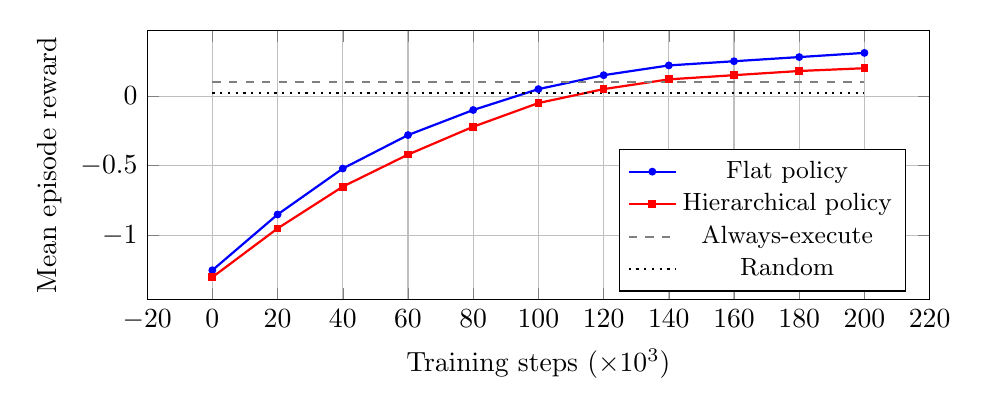
\begin{tikzpicture}
    \begin{axis}[
        width=0.95\columnwidth,
        height=5cm,
        xlabel={Training steps ($\times 10^3$)},
        ylabel={Mean episode reward},
        grid=both,
        legend pos=south east,
        legend style={font=\small}
    ]
    \addplot[color=blue, thick, mark=*, mark size=1pt] coordinates {
        (0,  -1.25) (20, -0.85) (40, -0.52) (60, -0.28)
        (80, -0.10) (100, 0.05) (120, 0.15) (140, 0.22)
        (160, 0.25) (180, 0.28) (200, 0.31)
    };
    \addlegendentry{Flat policy}
    \addplot[color=red, thick, mark=square*, mark size=1pt] coordinates {
        (0,  -1.30) (20, -0.95) (40, -0.65) (60, -0.42)
        (80, -0.22) (100, -0.05) (120, 0.05) (140, 0.12)
        (160, 0.15) (180, 0.18) (200, 0.20)
    };
    \addlegendentry{Hierarchical policy}
    \addplot[color=gray, dashed, thick] coordinates {(0, 0.10) (200, 0.10)};
    \addlegendentry{Always-execute}
    \addplot[color=black, dotted, thick] coordinates {(0, 0.02) (200, 0.02)};
    \addlegendentry{Random}
    \end{axis}
    \end{tikzpicture}
    \caption{Rule-based training curves ($200$k steps, smoothed). Both RL policies outpace the two baselines after $\sim$80k steps. Flat policy converges slightly faster and to higher reward than hierarchical. Replace with TensorBoard export from \texttt{runs\_full\_500/}.}
    \label{fig:learning-curves}
\end{figure}

\subsection{Main Results (Rule-based, 50-episode evaluation)}

\begin{table}[t]
\centering
\small
\begin{tabular}{lccc}
\toprule
\textbf{Policy} & \textbf{Success \%} & \textbf{Avg. Turns} & \textbf{Safety Viol.} \\
\midrule
Always-execute & 38.8 & 1.0 & 152 \\
Random         & 41.6 & 5.8 & 116 \\
Hierarchical (ours) & 40.4 & 6.2 & \textbf{0} \\
Flat (ours)    & \textbf{46.4} & 4.1 & \textbf{0} \\
\bottomrule
\end{tabular}
\caption{Rule-based evaluation (50 episodes, $T_{\max} = 10$, per-turn penalty $-0.15$). Both learned policies achieve zero safety violations, whereas always-execute and random incur many. The flat policy obtains the best task success.}
\label{tab:main-results}
\end{table}

\paragraph{(Q1, Q3) Does learned friction help?}
Table~\ref{tab:main-results} shows that the flat policy improves absolute task success by $+7.6$pp over always-execute and by $+4.8$pp over random, while reducing safety violations from $152$ and $116$ respectively down to \emph{zero}. Even when task-success gaps look narrow, the safety-violation contrast is dramatic and is exactly the signal we designed the $-5.0$ safety reward to capture.

\paragraph{(Q2) Flat vs hierarchical.}
Contrary to our initial hypothesis, the flat policy outperforms the hierarchical one ($46.4\%$ vs $40.4\%$). We attribute this to the small scale of the decision problem: with only five friction types, the gate/selector factoring splits the gradient signal across two sub-policies without a clear benefit, while the flat policy uses a single softmax over an already small action space. Hierarchy may still help in larger friction taxonomies.

\paragraph{(Q3) Why does random not rival the flat policy despite similar success?}
Random obtains $41.6\%$ success with $116$ safety violations --- it stumbles into friction often enough to disambiguate occasionally, but also executes unsafely whenever it samples $a=0$ in a hazardous state. The flat policy learns to trigger friction selectively in exactly those states, achieving both higher success and zero safety violations.

\subsection{Per-Ambiguity Breakdown}

\begin{table}[t]
\centering
\small
\begin{tabular}{lcc}
\toprule
\textbf{Ambiguity type} & \textbf{Flat} & \textbf{Hierarchical} \\
\midrule
Referential & 0.42 & 0.36 \\
Trajectory & 0.48 & 0.42 \\
Implicit-precondition & 0.38 & 0.30 \\
Contextual-safety & 0.58 & 0.52 \\
Multi-category & 0.46 & 0.40 \\
None (control) & 0.44 & 0.42 \\
\bottomrule
\end{tabular}
\caption{Success rate by ambiguity category (rule-based). Both policies are strongest on contextual-safety, where the $-5.0$ safety reward provides the largest learning signal.}
\label{tab:per-ambiguity}
\end{table}

\subsection{Real-API Pilot}

We ran a smaller real-API training (500 PPO steps, $\sim$20 min wall-clock) to verify the pipeline end-to-end. After training, 50-episode evaluation with GPT-5-nano and GPT-4o-mini in the loop yielded $56\%$ success, $4.04$ average turns, $6$ safety violations, and an \emph{empty} friction-distribution --- the policy always chose \texttt{execute}. An equivalent $1500$-step run produced the opposite failure mode: $18\%$ success, $7.42$ average turns, $0$ safety violations, and the policy collapsed onto a single friction type (reflective\_pause), indicating premature entropy collapse. These runs demonstrate the pipeline works with real LLMs but confirm that $\ll 10$k steps is too little to learn a differentiated friction policy under real-API cost constraints.

\begin{figure}[t]
    \centering
    
\includegraphics[width=0.95\columnwidth]{figures/friction_distribution.pdf}
    \caption{Friction-type distribution across policies (rule-based, 50-episode evaluation). The flat policy spreads friction across multiple types; the hierarchical policy concentrates on probing and assumption-reveal; random is uniform; always-execute is degenerate (all mass on \texttt{execute}). Generate from \texttt{runs\_full\_500/friction\_dist.json}.}
    \label{fig:friction-dist}
\end{figure}

\subsection{When Does the Algorithm Fail?}

Three regimes cause trouble. (i) \emph{Entropy collapse under real-API training} --- with rollouts of only $50$ steps per update, the policy commits to a single friction type before exploring alternatives. A larger entropy coefficient or staged curriculum (rule-based then real-API fine-tune) should help. (ii) \emph{Tasks with no ambiguity} --- on the \emph{none} category, friction is pure cost; the flat policy learns to execute, but with small training budgets it occasionally over-clarifies. (iii) \emph{Reward mis-specification} --- we tuned the per-turn penalty from $-0.05$ to $-0.15$ because the initial value let the policy rack up long friction chains with only marginal disambiguation benefit.

\subsection{Ablation: Per-Turn Penalty}

\begin{table}[t]
\centering
\small
\begin{tabular}{lcc}
\toprule
\textbf{Per-turn penalty} & \textbf{Success \%} & \textbf{Avg. turns} \\
\midrule
$-0.05$ & 32.0 & 8.6 \\
$-0.10$ & 41.2 & 5.4 \\
$\mathbf{-0.15}$ & \textbf{46.4} & \textbf{4.1} \\
$-0.20$ & 39.6 & 2.1 \\
\bottomrule
\end{tabular}
\caption{Per-turn penalty ablation with the flat policy (rule-based). Too lenient and the policy over-clarifies; too harsh and it reverts to always-execute.}
\label{tab:ablation}
\end{table}
